%%%%%%%%%%%%%%%%%%%%%%%%%%%%%%%%%%%%%%%%%%%%%%%%%
% ACOSUS Paper: An AI-driven Transfer Student Advising System
% Document Class: Article with ACM-style formatting
%%%%%%%%%%%%%%%%%%%%%%%%%%%%%%%%%%%%%%%%%%%%%%%%%

\documentclass[a4paper,10.5pt,twoside]{article}
\hyphenpenalty=500
\tolerance=1000
\emergencystretch=3em
\textwidth=125mm
\textheight=200mm
\usepackage[top=3cm, bottom=3cm, inner=3cm, outer=3cm, includehead]{geometry}
\usepackage{fancyhdr}
\pagestyle{fancy}
\fancyhead{}
\fancyfoot{}
\raggedbottom
\usepackage{xurl}
\usepackage{graphicx}
\usepackage{alltt}
\usepackage{amsmath}
\usepackage{booktabs}
\usepackage[hidelinks, pdftex]{hyperref}
\usepackage{float}

% TikZ packages for diagrams
\usepackage{tikz}
\usetikzlibrary{shapes.geometric, arrows.meta, positioning, fit, backgrounds, calc}

% Define colors for diagrams
\definecolor{targetsurvey}{HTML}{FFF3E0}
\definecolor{factorsurvey}{HTML}{E3F2FD}
\definecolor{processing}{HTML}{F3E5F5}
\definecolor{outputgreen}{HTML}{E8F5E9}
\definecolor{stage1green}{HTML}{D4EDDA}
\definecolor{stage1border}{HTML}{28A745}
\definecolor{stage2yellow}{HTML}{FFF3CD}
\definecolor{stage2border}{HTML}{FFC107}
\definecolor{stage3blue}{HTML}{CCE5FF}
\definecolor{stage3border}{HTML}{007BFF}
\definecolor{framegray}{HTML}{F8F9FA}
\definecolor{frameborder}{HTML}{6C757D}
\definecolor{modelpink}{HTML}{FCE4EC}
% Colors for fig2 (Three-Stage Pipeline)
\definecolor{stage1}{RGB}{76,175,80}
\definecolor{stage2}{RGB}{255,152,0}
\definecolor{stage3}{RGB}{100,149,237}
\definecolor{inputred}{RGB}{183,28,28}
\definecolor{outputviolet}{RGB}{103,58,183}
\definecolor{pipelineborder}{RGB}{120,60,60}
% Colors for fig3 (Survey Processing)
\definecolor{surveyblue}{RGB}{66,133,244}
\definecolor{surveyboxfill}{RGB}{215,232,252}
\definecolor{processorange}{RGB}{234,67,53}
\definecolor{processboxfill}{RGB}{253,232,226}
\definecolor{processboxborder}{RGB}{230,150,100}
\definecolor{modelgreen}{RGB}{15,100,80}
\definecolor{modelboxfill}{RGB}{200,230,225}
\definecolor{modelboxborder}{RGB}{100,180,170}
% Colors for fig4 (System Architecture)
\definecolor{dblue}{RGB}{60,100,180}

% TikZ styles
\tikzset{
    surveybox/.style={rectangle, rounded corners=3pt, minimum width=2.2cm, minimum height=0.8cm, text centered, draw=black!60, font=\scriptsize, text width=2cm, align=center},
    groupbox/.style={rectangle, rounded corners=5pt, draw=black!40, thick},
    arrow/.style={-{Stealth[length=2mm]}, thick, black!70},
    dashedarrow/.style={-{Stealth[length=2mm]}, thick, black!50, dashed},
    stagebox/.style={rectangle, rounded corners=5pt, minimum width=3cm, minimum height=1.8cm, draw, thick, text width=2.8cm, align=center, font=\scriptsize},
    layerbox/.style={rectangle, rounded corners=3pt, minimum width=2cm, minimum height=0.6cm, text centered, draw=black!60, font=\tiny, text width=1.8cm, align=center},
}
\urlstyle{same}
\usepackage[T1]{fontenc}
\usepackage[utf8]{inputenc}
\usepackage{lmodern}
\usepackage{csquotes}
\usepackage[style=numeric, backend=biber, sorting=none]{biblatex}
\addbibresource{references.bib}
\pagenumbering{arabic}
\setcounter{page}{1}

\usepackage[english]{babel}

\begin{document}
\fancyhead[LE]{\thepage\ \ \ \ [Author Last Names]}
\fancyhead[RO]{ACOSUS: AI-driven Transfer Student Advising\ \ \ \ \thepage}

\begin{center}
\LARGE
\textbf{An AI-driven Transfer Student Advising System: Design, Implementation, and Evaluation}\\[12pt]
\normalsize
\textbf{Author1,\footnote{Author1 title, Author1 institution, Author1 country, Author1 email.} Author2,\footnote{Author2 title, Author2 institution, Author2 country, Author2 email.} and Author3\footnote{Author3 title, Author3 institution, Author3 country, Author3 email.}}\\[4pt]
\end{center}

\begin{abstract}
\normalsize
Transfer students---particularly those from underrepresented backgrounds in computing---run into problems that regular advising tools were not built to handle. Their records are scattered across schools, receiving universities have little access to their earlier coursework, and most prediction models were built for students who started as freshmen.

We built ACOSUS (AI-driven counseling system for transfer students), an advising platform made specifically for this group. The system has two key design decisions: a two-survey setup that keeps outcome measurement separate from data collection while giving advisors a single, combined view of each student, and a step-by-step learning approach that works around having little data from the start. In a pilot test with transfer students at a public urban university, participants confirmed that the survey process works smoothly and found the system both easy to use and useful. The system is now live and collecting data so we can evaluate its predictions in the future.\vskip 2mm
\textbf{Keywords:} transfer students, intelligent advising, machine learning, higher education, student success prediction.
\end{abstract}

%%%%%%%%%%%%%%%%%%%%%%%%%%%%%%%%%%%%%%%%%%%%%%%%%
% SECTION 1: INTRODUCTION
%%%%%%%%%%%%%%%%%%%%%%%%%%%%%%%%%%%%%%%%%%%%%%%%%
\section{Introduction}\label{sec:introduction}

More and more students are starting at community colleges and later transferring to four-year universities to finish their degrees. National studies estimate that over a third of all undergraduates take this route \cite{ishitani2018student,roksa2008credits}, and the share is even higher among STEM majors, first-generation students, low-income students, and students of color \cite{wali2025transfer,computingtransfer2024,jabbar2019complex}. While the community college path offers a cheaper way into a bachelor's degree \cite{socialcognitive2022,factoranalysis2023}, it creates real coordination problems for both the sending and receiving schools \cite{topicmodeling2024,factoranalysis2023}. Advisors at the four-year school have to work with unclear transfer credit rules, inconsistent credit acceptance, and little knowledge of what the student did before arriving \cite{nguyen2024community,roksa2008credits,preposttransfer2014}. For students from groups already underrepresented in STEM, these challenges pile on top of financial stress and the feeling of not belonging in their new environment \cite{computingtransfer2024,wang2020road,socialcognitive2022}.

Keeping transfer students enrolled and graduating on time is a major concern. These students are more likely than those who started as freshmen to experience ``transfer shock''---a temporary dip in GPA and sense of belonging during their first two semesters \cite{jaggars2025,laanan2010adjustment}---and they drop out at higher rates. Researchers have found that certain measurable factors---cumulative GPA, number of credits accepted, test scores, distance between schools, and financial aid---correlate with whether students stay and graduate \cite{wang2020road,factoranalysis2023,jaggars2025,thiry2023,townsend2009}. But these numbers alone miss important parts of the picture \cite{topicmodeling2024,socialcognitive2022}. Interview-based studies keep showing that social support, faculty mentorship, and campus involvement (like research assistantships or hackathons) also matter a great deal, and these are hard to capture in standard university databases \cite{topicmodeling2024,thiry2023}.

Good advising is one of the most important factors in whether transfer students succeed \cite{topicmodeling2024,preposttransfer2014,lukszo2020,thiry2023}. Students want clear, timely, personalized guidance, but advisors at many schools carry such heavy caseloads that they cannot dig into each student's background and goals \cite{topicmodeling2024,preposttransfer2014}. The dashboards advisors currently use mostly show registrar data and early-warning flags designed for students who started as freshmen. They rarely include a student's pre-transfer history, credit transfer details, or the kinds of information students share in conversations about their decision-making \cite{nguyen2024community,preposttransfer2014}. As a result, prediction models can get things wrong and widen existing inequities \cite{computingtransfer2024,socialcognitive2022}. There is a clear need for a broader approach---one that combines numbers with what transfer students actually experience \cite{topicmodeling2024,socialcognitive2022}.

To fill this gap, we designed and tested an intelligent advising system that combines academic records with social, financial, and experiential data collected before and after transfer. Our contributions:

\begin{enumerate}
    \item We built an advising platform specifically for transfer students that combines standard academic records with information students provide about their own backgrounds, creating a single longitudinal profile for each student.
    \item We designed a two-survey setup that keeps outcome measurement (Target Surveys) separate from data collection (Factor Surveys), allowing consistent collection of transfer-specific variables---academic background, financial situation, and logistics---while giving advisors structured student profiles through a single dashboard.
    \item We built a modular prediction system with extensive configuration options. The design is algorithm-agnostic---any compatible method can be plugged into each stage---so researchers can test different approaches on their own student populations. Configuration options for survey linkage, phase transitions, and hyperparameters allow customization without changing code.
    \item We tested the platform with transfer students, who gave feedback on their experience. Results show the system streamlines self-advising and is seen as trustworthy, actionable, and supportive of equity.
\end{enumerate}

The rest of the paper is organized as follows. Section~\ref{sec:literature} reviews related work on transfer student success and intelligent advising. Section~\ref{sec:methodology} describes our system design, methodology, and implementation. Section~\ref{sec:evaluation} reports results from our pilot study. Section~\ref{sec:conclusion} concludes and outlines future directions.

%%%%%%%%%%%%%%%%%%%%%%%%%%%%%%%%%%%%%%%%%%%%%%%%%
% SECTION 2: LITERATURE REVIEW
%%%%%%%%%%%%%%%%%%%%%%%%%%%%%%%%%%%%%%%%%%%%%%%%%
\section{Literature Review}\label{sec:literature}

Research on transfer student outcomes falls into two related areas \cite{factoranalysis2023}. The first looks at the personal and academic traits that shape a student's transfer experience. The second examines what schools do---especially through advising---to support (or fail to support) these students.

Early models, like Ty et al.'s use of Social-Cognitive Career Theory, describe transfer success in terms of ``person inputs'' (e.g., socioeconomic status, self-confidence) and ``transfer receptivity''---how welcoming and well-organized the receiving school is \cite{computingtransfer2024}. Studies across STEM programs show that students' self-confidence and goal-setting tend to improve after they move to a four-year school, even as they face unfamiliar academic expectations \cite{socialcognitive2022,topicmodeling2024}. Factor analysis studies confirm that finances, school reputation, distance from home, and family expectations all play into the initial decision to transfer \cite{factoranalysis2023}. Regression analyses link post-transfer GPA to race/ethnicity and first-generation status \cite{computingtransfer2024}. Topic modeling of open-ended survey and social media responses fills in more detail---students express frustration with how credits are evaluated, long commutes, and limited chances to get involved on campus \cite{topicmodeling2024}.

Advising research centers on ``transfer student capital''---the knowledge and connections students build as they move between schools \cite{laanan2010adjustment,lukszo2020}. When official advising falls short, many students turn to Reddit, Discord, or peer forums for help with financial aid, housing, and course selection \cite{topicmodeling2024,nguyen2024community}. Interviews show that relationship-based advising eases transfer shock and helps students feel like they belong \cite{thiry2023,jaggars2025}. But advisors themselves say they struggle to keep up with constantly changing transfer credit rules, especially with large caseloads \cite{preposttransfer2014,nguyen2024community}.

Some technology tools have started to appear, but most were designed for students who entered as freshmen \cite{nguyen2024community}. Typical prediction tools pull from registrar data and LMS (Learning Management Systems) clickstreams. They rarely account for transfer-specific factors like how quickly credits were completed or whether students feel they belong at their new school \cite{nguyen2024community,topicmodeling2024}. Researchers warn that models trained on one type of student population can produce biased results that hurt underrepresented students \cite{socialcognitive2022,computingtransfer2024}. Only a few prototype systems focus on transfer students specifically, and these are still small-scale \cite{topicmodeling2024,socialcognitive2022}.

Given this, researchers have called for mixed-methods approaches that combine quantitative data with richer qualitative information \cite{socialcognitive2022,wang2020road}. Topic modeling is one promising approach: it can pull out recurring themes from written survey responses to surface challenges that do not show up in numbers. Deng et al.\ used Revealed Causal Mapping on narrative responses to trace how social media use shapes academic experiences for first-generation students \cite{deng2021}. Thiry et al.\ used mixed-methods case studies to develop support strategies for STEM transfer students \cite{thiry2023}. But few studies have fed these kinds of unstructured findings back into automated advising tools.

A separate problem makes the technology gap even worse: data scarcity. Ironically, this is not because there are too few transfer students---it is because their records are split across different schools \cite{nguyen2024community,roksa2008credits}. When students transfer, only a thin slice of their academic record moves with them: credits earned, GPA, and course equivalencies. The deeper understanding that community college advisors build up over time---knowledge about family obligations, financial stress, career goals, and early warning signs---rarely makes it to the new school \cite{roksa2008credits,nguyen2024community}. This information either goes undocumented or stays locked in systems the receiving university cannot access \cite{preposttransfer2014,topicmodeling2024}. University advisors have to reconstruct this picture through time-consuming intake conversations. And machine learning systems face a cold-start problem: each university has to build its training data from scratch, one student at a time \cite{coleman2019coldstart}. Traditional prediction approaches struggle in these small-cohort settings \cite{coleman2019coldstart}, and the very factors that best predict success are exactly the ones that get lost in the transfer process \cite{socialcognitive2022,roksa2008credits}.

Our work addresses these gaps from a systems-design perspective. Building on earlier findings from both quantitative and qualitative research, we built an advising platform that combines standard academic records (transfer credits, GPA, enrollment status) with data students provide about their own experiences. A lightweight, interpretable classifier uses this combined data to generate personalized success predictions. A dashboard delivers these predictions directly to students. Early feedback from the pilot suggests the system fills a real gap in transfer student support and could serve as a model for other schools.

%%%%%%%%%%%%%%%%%%%%%%%%%%%%%%%%%%%%%%%%%%%%%%%%%
% SECTION 3: METHODOLOGY AND IMPLEMENTATION
%%%%%%%%%%%%%%%%%%%%%%%%%%%%%%%%%%%%%%%%%%%%%%%%%
\section{Methodology and Implementation}\label{sec:methodology}

This section covers how we designed and built the ACOSUS platform. We start with the overall architecture (\S\ref{subsec:sysarch}), then describe how we collect data through two types of surveys (\S\ref{subsec:dualsurvey}), explain how survey responses are processed (\S\ref{subsec:dataprocessing}), walk through the progressive learning framework for small-data settings (\S\ref{subsec:progressive}), and finish with the configuration options that let other institutions adapt the system (\S\ref{subsec:config}).

\subsection{System Architecture}\label{subsec:sysarch}

ACOSUS uses a four-layer design that splits responsibilities between the user interface, application logic, data storage, and prediction models (Figure~\ref{fig:architecture}). Each layer can be updated or scaled independently.

The \textbf{Presentation Layer} provides different web views for different users. Students can fill out surveys, see predictions, and leave feedback. Advisors see a dashboard that pulls together each student's profile---organized by the same categories as the surveys---so they do not have to hunt through multiple sources. Administrators can set up surveys, start model training, and check system stats.

The \textbf{Business Logic Layer} manages the application's workflows and controls when the system moves between phases of the progressive learning framework. It makes sure students see the right interface based on where the system currently is---data collection only during the early phase, predictions plus feedback in later phases.

The \textbf{Data Layer} stores users, surveys, responses, and model information in a flexible document database. Because the structure is flexible, researchers can change survey questions without needing to update the database schema.

The \textbf{Model Layer} runs as a separate service that handles the heavy lifting: normalizing data, making predictions across all three pipeline stages, and training models. Long training jobs run in background queues so they do not slow down prediction requests. Model versioning makes sure that new models only go live after they prove they perform better on real student data.

% Figure 1 - System Architecture diagram
\begin{figure}[htbp]
\centering
\resizebox{0.95\textwidth}{!}{%
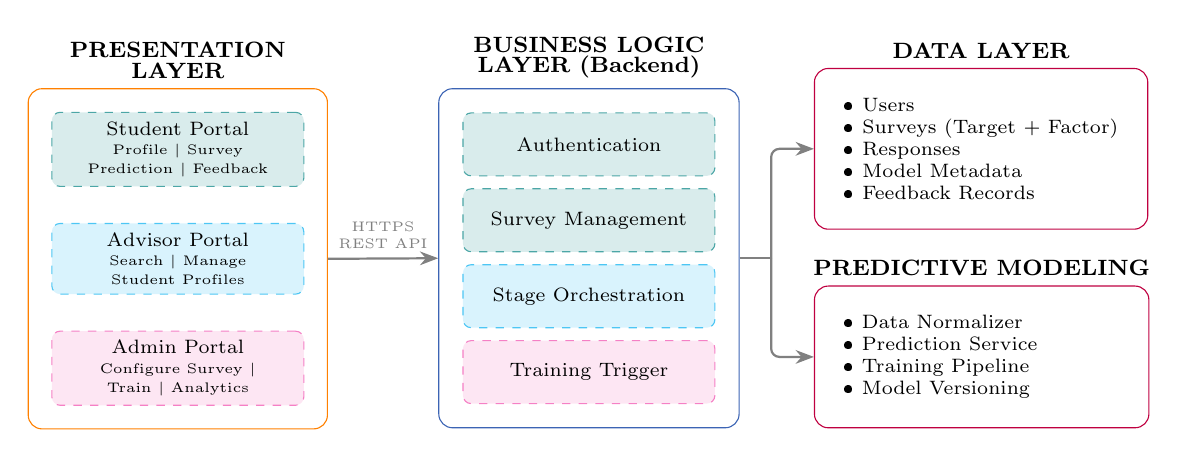
\begin{tikzpicture}[
    node distance=1.5mm,
    box/.style={draw, dashed, rounded corners=3pt, minimum width=32mm, minimum height=8mm, align=center, font=\scriptsize},
    layer/.style={draw, rounded corners=5pt, inner sep=3mm},
    student/.style={box, draw=teal!70, fill=teal!15},
    advisor/.style={box, draw=cyan!70, fill=cyan!15},
    admin/.style={box, draw=magenta!50, fill=magenta!10},
    lbl/.style={font=\footnotesize\bfseries, align=center},
    >=Stealth
]

% Column 2: Business Logic Layer (reference)
\node[student] (auth) {Authentication};
\node[student, below=of auth] (surv) {Survey Management};
\node[advisor, below=of surv] (stage) {Stage Orchestration};
\node[admin, below=of stage] (train) {Training Trigger};

\begin{scope}[on background layer]
\node[layer, draw=dblue, fit=(auth)(surv)(stage)(train), label={[lbl]above:BUSINESS LOGIC\\[-2pt]LAYER (Backend)}] (biz) {};
\end{scope}

% Column 1: Presentation Layer - create outer box first, then place inner boxes
\path let \p1=(biz.north), \p2=(biz.south), \p3=(biz.west) in
    node[layer, draw=orange,
         minimum height={\y1-\y2},
         minimum width=38mm,
         anchor=north east,
         label={[lbl]above:PRESENTATION\\[-2pt]LAYER}] (pres) at ($(\x3,\y1)+(-14mm,0)$) {};

% Place boxes centered inside pres
\node[student, anchor=north] at ($(pres.north)+(0,-3mm)$) (sp) {Student Portal\\[-1pt]\tiny Profile \textbar{} Survey\\[-1pt]\tiny Prediction \textbar{} Feedback};
\node[advisor] at (pres.center) (ap) {Advisor Portal\\[-1pt]\tiny Search \textbar{} Manage\\[-1pt]\tiny Student Profiles};
\node[admin, anchor=south] at ($(pres.south)+(0,3mm)$) (adm) {Admin Portal\\[-1pt]\tiny Configure Survey \textbar{} \\[-1pt]\tiny Train \textbar{} Analytics};

% Column 3: Data Layer (top) + ML Layer (bottom)
% Position Data Layer at top, aligned with Business Logic Layer outer box
\path let \p1=(biz.north east) in
    node[font=\scriptsize, align=left, anchor=north west] (dlist) at ($(\x1,\y1)+(12mm,0)$) {
        \textbullet\ Users\\
        \textbullet\ Surveys (Target + Factor)\\
        \textbullet\ Responses\\
        \textbullet\ Model Metadata\\
        \textbullet\ Feedback Records
    };

\begin{scope}[on background layer]
\node[layer, draw=purple, fit=(dlist), inner sep=2.5mm, label={[lbl]above:DATA LAYER}] (data) {};
\end{scope}

% Predictive Modeling Layer - align bottom with Business Logic Layer
\path let \p1=(data.west), \p2=(data.east), \p3=(biz.south) in
    node[layer, draw=purple, minimum width={\x2-\x1}, minimum height=18mm, anchor=south west, label={[lbl]above:PREDICTIVE MODELING}] (ml) at (\x1,\y3) {};

\node[font=\scriptsize, align=left, anchor=north west] at ($(ml.north west)+(2.5mm,-2.5mm)$) {
    \textbullet\ Data Normalizer\\
    \textbullet\ Prediction Service\\
    \textbullet\ Training Pipeline\\
    \textbullet\ Model Versioning
};

% Arrows
\draw[->, thick, gray] (pres.east) -- (biz.west) node[midway, above, font=\tiny, align=center] {HTTPS\\REST API};
\coordinate (split) at ($(biz.east)+(4mm,0)$);
\draw[thick, gray] (biz.east) -- (split);
\draw[->, thick, gray, rounded corners=3pt] (split) |- (data.west);
\draw[->, thick, gray, rounded corners=3pt] (split) |- (ml.west);

\end{tikzpicture}
}%
\caption{ACOSUS system architecture. Four layers separate presentation, business logic, data persistence, and predictive modeling, enabling independent scaling and clear separation of responsibilities.}
\label{fig:architecture}
\end{figure}

\subsection{Dual-Survey Architecture}\label{subsec:dualsurvey}

First, we define some key terms used throughout this paper. ACOSUS sets up transfer student success prediction as a standard prediction problem: given a set of input variables, predict an outcome. We use these terms:

\begin{itemize}
    \item \textbf{Target Survey / Outcome ($Y$)}: The survey instrument that measures what we want to predict---the student's likelihood of academic success. In machine learning terminology, this is the \emph{label} or \emph{dependent variable}.
    \item \textbf{Factor Survey / Predictors ($X$)}: The survey instruments that collect information used to make predictions---academic background, financial circumstances, and logistical constraints. In machine learning terminology, these are \emph{features} or \emph{independent variables}.
    \item \textbf{Constructs}: Psychological or educational concepts (e.g., self-efficacy, institutional commitment) that we measure through survey questions. A single Factor Survey may cover several constructs.
\end{itemize}

The factors that best predict transfer success---how credits transfer, how severe ``transfer shock'' is, whether students feel they belong, and whether they are financially stable---are usually missing from standard university systems \cite{topicmodeling2024,computingtransfer2024,socialcognitive2022}. On top of that, advisors do not have easy access to the information they need. Research shows that advisors spend a lot of time gathering data from scattered sources before they can give useful advice \cite{preposttransfer2014,thiry2023}. ACOSUS tackles both problems with a two-survey design that feeds the AI model and brings together the information advisors need in one place.

Previous research has found that transfer student success depends on multiple factors: academic confidence, commitment to the school, social connections, and clear career goals \cite{factoranalysis2023,topicmodeling2024,computingtransfer2024}. Our own earlier factor analysis identified clusters of variables---academic confidence, time management, financial stability, and support networks---that separate successful transfer students from those who struggle \cite{factoranalysis2023}. Building on this, ACOSUS defines ``success'' as the student's overall likelihood of doing well across these areas, and ``factors'' as the things that affect that likelihood.

The system uses two types of surveys to collect this data separately. \textbf{Target Surveys} (measuring $Y$) capture success in one of two ways: (1) a single question where students rate their success on a 0--100 scale, or (2) a multi-question instrument covering constructs like academic confidence, commitment, time management, and career motivation, which get combined into one score. \textbf{Factor Surveys} (measuring $X$) collect the predictor variables, organized into groups: academic background (pre-transfer GPA, transferred credits, test scores), financial situation (scholarships, family support, employment), logistics (commute distance, work hours), and interests/experience (career goals, prior subject experience).

Beyond feeding the AI model, Factor Surveys solve a practical problem for advisors: they make sure every transfer student answers the same questions. This means advisors can compare across students, and no important risk factor gets missed. Responses show up immediately in the advisor dashboard---no need to search through emails, notes, or schedule follow-up meetings.

The system also supports flexible study designs through \textbf{survey linkage}---direct links between Target and Factor Surveys. This lets researchers compare different predictor sets, adapt to new factors, and customize for different student groups without changing the underlying system. Section~\ref{subsec:config} explains how this works in practice.

% Figure 3 - Dual-Survey Architecture diagram
\begin{figure}[htbp]
\centering
\resizebox{0.95\textwidth}{!}{%
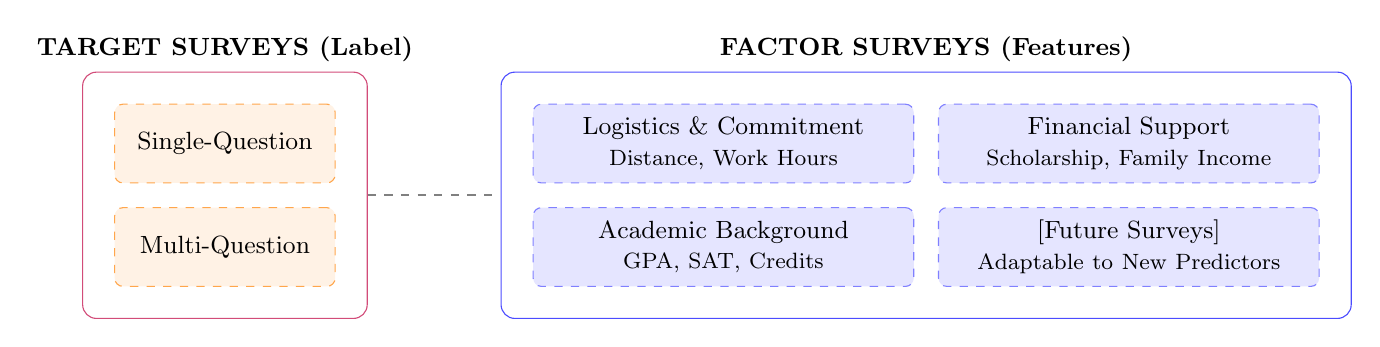
\begin{tikzpicture}[
  box/.style={draw,dashed,rounded corners=3pt,align=center,font=\small},
  target/.style={box,draw=orange!70,fill=orange!10,minimum width=28mm,minimum height=10mm},
  factor/.style={box,draw=blue!50,fill=blue!10,minimum width=48mm,minimum height=10mm,text width=46mm},
  container/.style={draw,rounded corners=5pt,inner sep=4mm}
]
% Target surveys
\node[target] (sq) {Single-Question};
\node[target,below=3mm of sq] (mq) {Multi-Question};
\node[container,draw=purple!70,fit=(sq)(mq),label={[font=\small\bfseries]above:TARGET SURVEYS (Label)}] (tbox) {};

% Factor surveys
\node[factor,right=25mm of sq] (lc) {Logistics \& Commitment\\\footnotesize Distance, Work Hours};
\node[factor,right=3mm of lc] (fs) {Financial Support\\\footnotesize Scholarship, Family Income};
\node[factor,below=3mm of lc] (ab) {Academic Background\\\footnotesize GPA, SAT, Credits};
\node[factor,right=3mm of ab] (fu) {[Future Surveys]\\\footnotesize Adaptable to New Predictors};
\node[container,draw=blue!70,fit=(lc)(fs)(ab)(fu),label={[font=\small\bfseries]above:FACTOR SURVEYS (Features)}] (fbox) {};

% Connection
\draw[gray,dashed,thick] (tbox.east) -- (fbox.west);
\end{tikzpicture}
}%
\caption{Dual-Survey Architecture. Target Surveys collect the outcome ($Y$), Factor Surveys collect predictors ($X$). Dashed lines show linkage relationships enabling flexible study configurations.}
\label{fig:dualsurvey}
\end{figure}

\subsection{Survey Data Processing}\label{subsec:dataprocessing}

The surveys described in Section~\ref{subsec:dualsurvey} turn student answers into numbers that the prediction model can use. Each question stands in for a success factor identified in earlier research---our factor analysis mapped observable things (like scholarship status or commute distance) to underlying concepts (like financial stability or school commitment) that predict outcomes \cite{factoranalysis2023}.

\subsubsection{Priority Weighting}

Not all factors matter equally. Research consistently shows that some variables---academic self-confidence, financial stability, institutional fit---predict success more strongly than others \cite{factoranalysis2023,computingtransfer2024,socialcognitive2022}. ACOSUS handles this through \textbf{priority scores}: each question gets a weight based on how important that factor is, drawing on effect sizes and factor loadings from prior studies. These weights can be updated as advisors learn which factors matter most at their school.

The weighted score calculation is straightforward. For a survey with $n$ questions, where question $i$ has priority $p_i$ and the student picks an option worth $w_i^{\text{selected}}$ out of a maximum $w_i^{\text{max}}$:

\begin{equation}
S = \frac{\sum_{i=1}^{n} \left(\frac{w_i^{\text{selected}}}{w_i^{\text{max}}} \times p_i\right)}{\sum_{i=1}^{n} p_i}
\label{eq:priority}
\end{equation}

This gives a score between 0 and 1 that accounts for both how good the student's answers are and how important each question is. We then apply a logistic curve to keep predictions from being too extreme at the high and low ends.

\begin{table}[htbp]
\centering
\caption{Example priority score assignments based on literature-informed importance.}
\label{tab:priority}
\begin{tabular}{@{}p{3.1cm}p{4.5cm}cp{3.5cm}@{}}
\toprule
\textbf{Factor Category} & \textbf{Example Question} & \textbf{Priority} & \textbf{Rationale} \\
\midrule
Academic ~ ~ ~ ~ ~ ~ ~ ~ ~ Self-Efficacy & How confident in your ability to succeed? & 9 & Strong predictor \cite{bandura1997} \\
\midrule
Financial Stability & Expected financial stress impact? & 8 & Affects retention \cite{socialcognitive2022} \\
\midrule
Institutional Commitment & How committed to completing this program? & 9 & Persistence indicator \cite{tinto1993} \\
\midrule
Logistics & Commute distance to university? & 6 & Practical barrier \\
\bottomrule
\end{tabular}
\end{table}

These priority weights have another benefit: they can serve as starting points (priors) when we move to more advanced probabilistic models. Features with higher priority get more initial influence, which the model can then adjust based on real data. This connects expert knowledge to learned parameters in a principled way.

\subsubsection{Data Type Handling}

Survey answers come in different types, and each type needs to be converted to numbers differently. The key distinction is between \textbf{ordinal} data (answers with a natural order, like ``Not confident'' $<$ ``Somewhat confident'' $<$ ``Very confident'') and \textbf{cardinal} data (categories without ranking, like career field choices).

\begin{table}[htbp]
\centering
\caption{Normalization strategies for different data types.}
\label{tab:normalization}
\begin{tabular}{@{}lll@{}}
\toprule
\textbf{Data Type} & \textbf{Example} & \textbf{Normalization Method} \\
\midrule
Ordinal & GPA range: ``3.0--3.5'' & Direct option weightage (e.g., 8/10) \\
Cardinal & Career: ``Industry/Corporate'' & Equal weightage or domain-specific mapping \\
Continuous & SAT score: 1250 & Min-max scaling: $(x - \min)/(\max - \min)$ \\
\bottomrule
\end{tabular}
\end{table}

This approach makes sure ordinal answers stay ordered, categorical answers are not falsely ranked, and continuous values are properly scaled.

% Figure 3 - Survey Data Processing Pipeline diagram
\begin{figure}[htbp]
\centering
\resizebox{0.95\textwidth}{!}{%
\begin{tikzpicture}[
    node distance=0.35cm,
    inner/.style={rectangle, dashed, thick, rounded corners=3pt, align=center, inner sep=10pt, font=\normalsize},
    outer/.style={rectangle, thick, rounded corners=3pt, inner sep=6pt},
    arrow/.style={-{Stealth[scale=0.9]}, gray!70, thick, rounded corners=6pt},
    arrowline/.style={gray!70, thick, rounded corners=6pt}
]

% Survey Collection inner boxes
\node[inner, fill=surveyboxfill, draw=surveyblue!70, text width=4cm, minimum height=0.5cm] (q1) {Question 1 (Ordinal)};
\node[inner, fill=surveyboxfill, draw=surveyblue!70, text width=4cm, minimum height=.5cm, below=0.2cm of q1] (q2) {Question 2 (Cardinal)};
\node[inner, fill=surveyboxfill!40, draw=surveyblue!40, densely dotted, text width=4cm, minimum height=.5cm, below=0.2cm of q2] (qdots) {\textit{...}};
\node[inner, fill=surveyboxfill, draw=surveyblue!70, text width=4cm, minimum height=0.5cm, below=0.2cm of qdots] (qn) {Question N (Continuous)};

% Survey Collection title and outer box
\node[above=0.3cm of q1, font=\normalsize\bfseries, text=surveyblue!80!black] (survey-title) {SURVEY COLLECTION};
\node[outer, draw=surveyblue, fit=(survey-title)(q1)(q2)(qdots)(qn), inner sep=10pt] (survey-box) {};

% Data Processing inner boxes
\node[inner, fill=processboxfill, draw=processboxborder, text width=3cm, minimum height=1cm, right=1.8cm of q1.east |- q1.south east] (priority) {Priority\\Weighting};
\node[inner, fill=processboxfill, draw=processboxborder, text width=3cm, minimum height=1cm, below=0.8cm of priority] (normalize) {Type-Aware\\Normalization};

% Data Processing title and outer box
\node[above=0.3cm of priority, font=\normalsize\bfseries, text=processorange!80!black] (process-title) {DATA PROCESSING};
\node[outer, draw=processorange, fit=(process-title)(priority)(normalize), inner sep=10pt] (process-box) {};

% Model Input inner box (centered with process box)
\path (priority.center) -- (normalize.center) coordinate[midway] (process-center);
\node[inner, fill=modelboxfill, draw=modelboxborder, text width=3cm, minimum height=1cm, right=1.5cm of process-box.east, anchor=west] (feature) {Normalized\\Feature Vector};

% Model Input title and outer box
\node[above=0.3cm of feature, font=\normalsize\bfseries, text=modelgreen] (model-title) {MODEL INPUT};
\node[outer, draw=modelgreen, fit=(model-title)(feature), inner sep=10pt] (model-box) {};

% Arrows from Survey to Priority Weighting (converging)
% Merge point at Q2 level so Q2 has straight horizontal line
\coordinate (merge-point) at ($(survey-box.east)!0.5!(process-box.west) |- q2$);

% Curved lines from questions converging to merge point, then to priority
\draw[arrowline] (q1.east) to[out=0, in=135] (merge-point);
\draw[arrowline] (q2.east) -- (merge-point);
\draw[arrowline] (qn.east) to[out=0, in=-135] (merge-point);
\draw[arrow] (merge-point) to[out=45, in=180] (priority.west);

% Arrow between Priority and Normalization
\draw[arrow] (priority.south) -- (normalize.north);

% Arrow from Normalization to Feature Vector
\draw[arrowline] (normalize.east) -- (process-box.east |- normalize.east);
\draw[arrow] (process-box.east |- normalize.east) to[out=0, in=180] (feature.west);

\end{tikzpicture}
}%
\caption{Survey data processing pipeline. Raw responses undergo priority weighting and type-aware normalization to produce standardized feature vectors for model ingestion.}
\label{fig:processing}
\end{figure}

\subsection{Progressive Learning Framework}\label{subsec:progressive}

ACOSUS is built to work with limited data from the start. Rather than waiting until enough data exists to make predictions, the system is useful from day one---even before any model is trained, advisors get structured student profiles through the standardized surveys. This means the early period when data is still being collected is not wasted time; it is a productive phase where advisors already benefit.

\subsubsection{Three-Stage Pipeline}

As more student data comes in, the system's prediction ability improves through three stages:

\textbf{Foundation Stage.} The system focuses on collecting high-quality labeled data through the survey instruments. Once enough observations exist, simple prediction methods generate initial results. At this stage, the priority is getting good data, not making sophisticated predictions.

\textbf{Augmentation Stage.} As the dataset grows, the system uses generative methods to create realistic synthetic data that expands the training set. These methods learn the patterns in the real data and produce additional samples that preserve the same statistical properties. This gives the system enough data to support more advanced algorithms.

\textbf{Refinement Stage.} With a larger training set (real + synthetic), the system switches to advanced nonlinear models that can capture complex relationships between features and outcomes.

The framework is modular: each stage is a swappable component. Any prediction method can serve Stage~1, any data generation technique can serve Stage~2, and any deep learning model can serve Stage~3. We call this an algorithm-agnostic design, and it serves two purposes. First, researchers can compare different algorithms to find what works best for their specific students, rather than being locked into one approach. Second, as new methods emerge in few-shot learning, data augmentation, or neural network design, they can be plugged in without redesigning the system. This makes ACOSUS a flexible framework that can adapt to diverse educational prediction contexts.

% Figure 4 - Three-Stage Progressive Pipeline diagram
\begin{figure}[htbp]
\centering
\resizebox{\textwidth}{!}{%
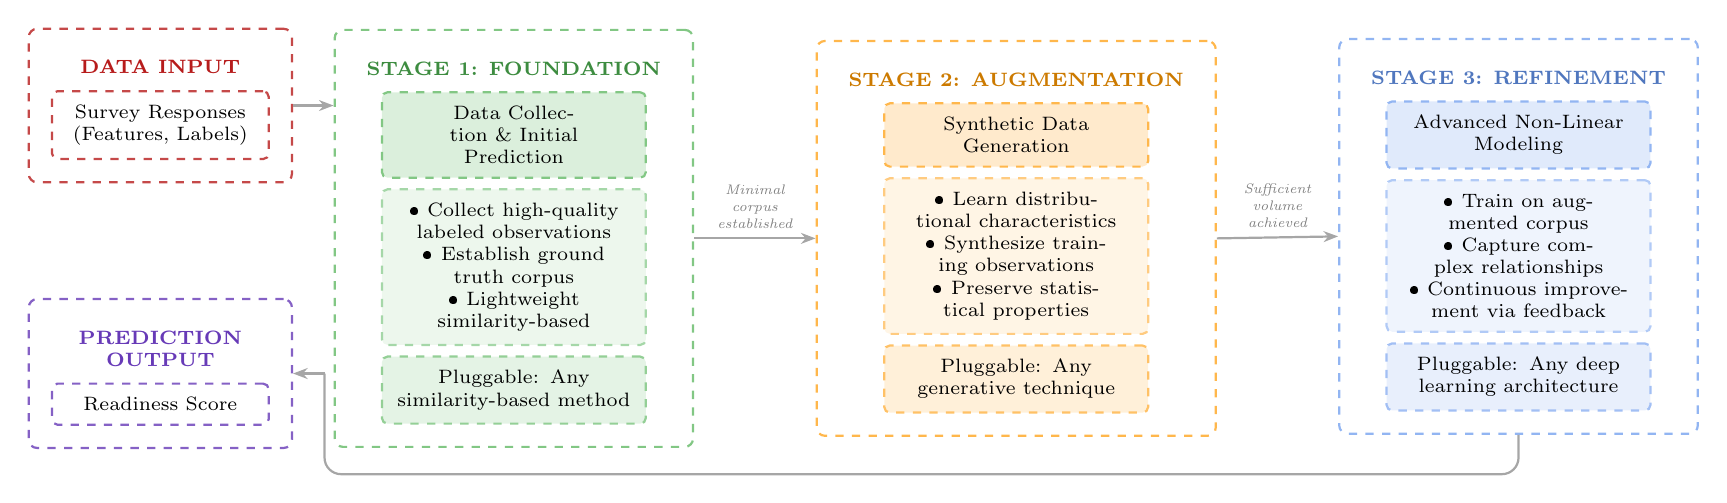
\begin{tikzpicture}[
    node distance=0.3cm,
    inner/.style={rectangle, dashed, thick, rounded corners=2pt, align=center, inner sep=5pt, font=\scriptsize},
    outer/.style={rectangle, dashed, thick, rounded corners=3pt, inner sep=8pt},
    header/.style={inner, fill=#1!20, draw=#1!70},
    content/.style={inner, fill=#1!10, draw=#1!50},
    plug/.style={inner, fill=#1!15, draw=#1!60},
    arrow/.style={-{Stealth[scale=0.8]}, gray!70, thick},
    lbl/.style={font=\tiny\itshape, text=gray, align=center}
]

% Stage 1 inner boxes
\node[header=stage1, text width=3cm, minimum height=0.8cm] (s1-head) {Data Collection \& Initial\\Prediction};
\node[content=stage1, below=0.12cm of s1-head, text width=3cm, minimum height=1.4cm] (s1-content) {
    \textbullet\ Collect high-quality labeled observations\\
    \textbullet\ Establish ground truth corpus\\
    \textbullet\ Lightweight similarity-based
};
\node[plug=stage1, below=0.12cm of s1-content, text width=3cm, minimum height=0.7cm] (s1-plug) {Pluggable: Any\\similarity-based method};
\node[above=0.08cm of s1-head, font=\scriptsize\bfseries, text=stage1!80!black] (s1-title) {STAGE 1: FOUNDATION};
\node[outer, draw=stage1!70, fit=(s1-title)(s1-head)(s1-content)(s1-plug)] (stage1-box) {};

% Stage 2 inner boxes
\node[header=stage2, right=3cm of s1-head, text width=3cm, minimum height=0.8cm] (s2-head) {Synthetic Data\\Generation};
\node[content=stage2, below=0.12cm of s2-head, text width=3cm, minimum height=1.4cm] (s2-content) {
    \textbullet\ Learn distributional characteristics\\
    \textbullet\ Synthesize training observations\\
    \textbullet\ Preserve statistical properties
};
\node[plug=stage2, below=0.12cm of s2-content, text width=3cm, minimum height=0.7cm] (s2-plug) {Pluggable: Any\\generative technique};
\node[above=0.08cm of s2-head, font=\scriptsize\bfseries, text=stage2!80!black] (s2-title) {STAGE 2: AUGMENTATION};
\node[outer, draw=stage2!70, fit=(s2-title)(s2-head)(s2-content)(s2-plug)] (stage2-box) {};

% Stage 3 inner boxes
\node[header=stage3, right=3cm of s2-head, text width=3cm, minimum height=0.8cm] (s3-head) {Advanced Non-Linear\\Modeling};
\node[content=stage3, below=0.12cm of s3-head, text width=3cm, minimum height=1.4cm] (s3-content) {
    \textbullet\ Train on augmented corpus\\
    \textbullet\ Capture complex relationships\\
    \textbullet\ Continuous improvement via feedback
};
\node[plug=stage3, below=0.12cm of s3-content, text width=3cm, minimum height=0.7cm] (s3-plug) {Pluggable: Any deep\\learning architecture};
\node[above=0.08cm of s3-head, font=\scriptsize\bfseries, text=stage3!80!black] (s3-title) {STAGE 3: REFINEMENT};
\node[outer, draw=stage3!70, fit=(s3-title)(s3-head)(s3-content)(s3-plug)] (stage3-box) {};

% Pipeline title (centered above stages)
% \path (stage1-box.north west) -- (stage3-box.north east) coordinate[midway] (pipeline-center);
% \node[above=0.6cm of pipeline-center, font=\small\bfseries, text=pipelineborder] (pipeline-title) {ACOSUS THREE-STAGE PROGRESSIVE PIPELINE};

% Pipeline outer box
% \begin{scope}[on background layer]
% \node[outer, draw=pipelineborder, fit=(pipeline-title)(stage1-box)(stage2-box)(stage3-box), inner sep=12pt] (pipeline) {};
% \end{scope}

% Input box (outer box top aligned with Stage 1 outer box top)
\node[font=\scriptsize\bfseries, text=inputred, anchor=north] (input-title) at ([xshift=-2.2cm, yshift=-8pt]stage1-box.north west) {DATA INPUT};
\node[inner, fill=white, draw=inputred!80, text width=2.4cm, below=0.08cm of input-title] (input-inner) {Survey Responses\\(Features, Labels)};
\node[outer, draw=inputred!80, fit=(input-title)(input-inner)] (input-box) {};

% Output box (outer box bottom aligned with Stage 1 outer box bottom)
\node[inner, fill=white, draw=outputviolet!80, text width=2.4cm, anchor=south] (output-inner) at ([xshift=-2.2cm, yshift=8pt]stage1-box.south west) {Readiness Score};
\node[above=0.08cm of output-inner, font=\scriptsize\bfseries, text=outputviolet, align=center] (output-title) {PREDICTION\\ OUTPUT};
\node[outer, draw=outputviolet!80, fit=(output-title)(output-inner)] (output-box) {};

% Arrows
\draw[arrow] (input-box.east) -- (stage1-box.west |- input-box.east);
\draw[arrow] (stage1-box.east) -- node[lbl, above] {Minimal\\corpus\\established} (stage2-box.west);
\draw[arrow] (stage2-box.east) -- node[lbl, above] {Sufficient\\volume\\achieved} (stage3-box.west);

% Feedback arrow
\coordinate (turn1) at ([yshift=-0.5cm]stage3-box.south);
\coordinate (turn2) at (turn1 -| output-box.east);
\coordinate (turn3) at ([xshift=0.4cm]output-box.east);
\draw[gray!70, thick, rounded corners=6pt] (stage3-box.south) -- (turn1) -- (turn1 -| turn3) -- (turn3);
\draw[arrow] (turn3) -- (output-box.east);

\end{tikzpicture}
}%
\caption{The Three-Stage Progressive Pipeline. Each stage represents a pluggable component that can be substituted with alternative algorithms. The framework progresses from data acquisition through augmentation to refined prediction, with feedback loops enabling continuous improvement.}
\label{fig:pipeline}
\end{figure}

\subsection{Configuration Flexibility}\label{subsec:config}

The flexible design from Section~\ref{subsec:progressive} is built into a configuration system that lets researchers adapt the framework without touching the core code. There are four areas of configuration:

\textbf{Survey Linkage:} The two-survey setup from Section~\ref{subsec:dualsurvey} works through link settings: a single Target Survey (outcome $Y$) can be connected to multiple Factor Surveys (predictor sets $X_1, X_2, X_3$). This lets researchers test which combination of predictors best predicts success. Specific benefits:

\begin{enumerate}
    \item \textbf{Comparing predictor sets}---deploy different Factor Surveys to the same group of students and compare which one predicts better;
    \item \textbf{Adding new factors over time}---as research identifies new predictors (e.g., post-pandemic stressors, new measures of transfer shock), new Factor Surveys can be added without breaking ongoing data collection or invalidating past comparisons;
    \item \textbf{Customizing by program}---different departments can use program-specific Factor Surveys (e.g., technical preparation for CS majors) while sharing a common outcome measure.
\end{enumerate}

% Figure 5 - Dual-Survey Architecture with Linkage
\begin{figure}[htbp]
\centering
\resizebox{0.95\textwidth}{!}{%
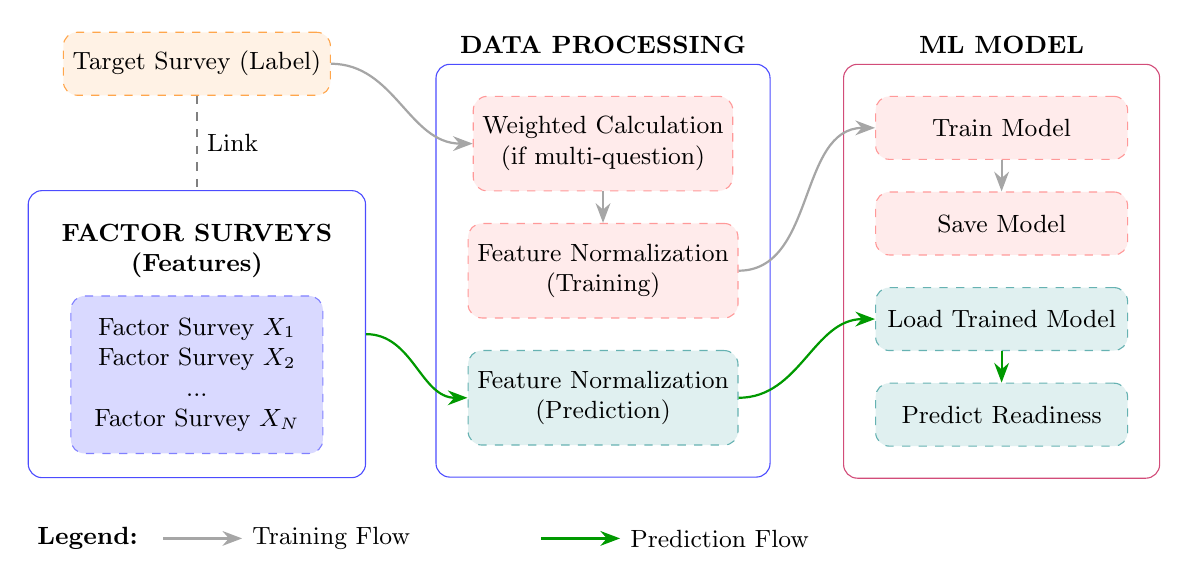
\begin{tikzpicture}[
  box/.style={draw,dashed,rounded corners=5pt,align=center,font=\small},
  container/.style={draw,rounded corners=5pt,inner sep=4mm},
  % Training flow styles (warm/salmon hues)
  trainbox/.style={box,draw=red!40,fill=red!8},
  trainarr/.style={gray!70,thick,-{Stealth[length=2.5mm]}},
  % Prediction flow styles (cool/teal hues)
  predbox/.style={box,draw=teal!60,fill=teal!12},
  predarr/.style={green!60!black,thick,-{Stealth[length=2.5mm]}}
]
% Left column - Target Survey
\node[box,draw=orange!70,fill=orange!10,minimum width=32mm,minimum height=8mm] (target) {Target Survey (Label)};

% Middle column - Data Processing
\node[trainbox,minimum width=32mm,minimum height=12mm,right=18mm of target.south east,anchor=north west] (weighted) {Weighted Calculation\\(if multi-question)};
\node[trainbox,minimum width=32mm,minimum height=12mm,below=4mm of weighted] (normtrain) {Feature Normalization\\(Training)};
\node[predbox,minimum width=32mm,minimum height=12mm,below=4mm of normtrain] (normpred) {Feature Normalization\\(Prediction)};
\node[container,draw=blue!70,fit=(weighted)(normtrain)(normpred),label={[font=\small\bfseries]above:DATA PROCESSING}] (dbox) {};

% Left column - Factor Surveys (aligned to dbox bottom)
\node[box,draw=blue!50,fill=blue!15,minimum width=32mm,minimum height=20mm,anchor=south] at ([yshift=3mm]target.south|-dbox.south) (factors) {Factor Survey $X_1$\\Factor Survey $X_2$\\...\\Factor Survey $X_N$};
\node[font=\small\bfseries,align=center,above=1mm of factors] (flabel) {FACTOR SURVEYS\\(Features)};
\node[container,draw=blue!70,inner sep=3mm,fit=(factors)(flabel)] (fbox) {};

% Link between target and factor surveys
\draw[gray,dashed,thick] (target.south) -- node[right,font=\small,black]{Link} (fbox.north);

% Right column - ML Model (Training flow on top, Prediction flow on bottom)
\node[trainbox,minimum width=32mm,minimum height=8mm,right=18mm of weighted.north east,anchor=north west] (train) {Train Model};
\node[trainbox,minimum width=32mm,minimum height=8mm,below=4mm of train] (save) {Save Model};
\node[predbox,minimum width=32mm,minimum height=8mm,below=4mm of save] (load) {Load Trained Model};
\node[predbox,minimum width=32mm,minimum height=8mm,below=4mm of load] (predict) {Predict Readiness};
\node[container,draw=purple!70,fit=(train)(save)(load)(predict),label={[font=\small\bfseries]above:ML MODEL}] (mbox) {};

% Training Flow Arrows (gray)
\draw[trainarr] (target.east) to[out=0,in=180] (weighted.west);
\draw[trainarr] (weighted.south) -- (normtrain.north);
\draw[trainarr] (normtrain.east) to[out=0,in=180] (train.west);
\draw[trainarr] (train.south) -- (save.north);

% Prediction Flow Arrows (green)
\draw[predarr] (fbox.east) to[out=0,in=180] (normpred.west);
\draw[predarr] (normpred.east) to[out=0,in=180] (load.west);
\draw[predarr] (load.south) -- (predict.north);

% Legend (horizontal layout)
\node[below=5mm of fbox.south west,anchor=north west,font=\small\bfseries] (legendlabel) {Legend:};
\draw[trainarr] ([xshift=2mm]legendlabel.east) -- ++(10mm,0) node[right,font=\small,black] {Training Flow};
\node[right=50mm of legendlabel.east,anchor=west] (predlegendstart) {};
\draw[predarr] (predlegendstart.west) -- ++(10mm,0) node[right,font=\small,black] {Prediction Flow};
\end{tikzpicture}
}%
\caption{Dual-Survey Architecture with survey linkage. Gray arrows indicate training flow (Target Survey through model training), while green arrows indicate prediction flow (Factor Surveys through inference). Dashed lines show linkage relationships between Target and Factor Surveys.}
\label{fig:linkage}
\end{figure}

The other three areas cover the progressive learning pipeline:

\textbf{Phase Transition Thresholds.} Administrators set how many observations trigger the jump from one pipeline stage to the next. Defaults are based on statistical rules of thumb for each type of algorithm, but schools can adjust based on their enrollment patterns and how they want to balance prediction availability against model reliability.

\textbf{Algorithm Selection:} Each pipeline stage accepts any algorithm that fits the required interface. Stage~1 needs a method that works with very little data (any similarity-based or instance-based method). Stage~2 needs a generative model that can create realistic synthetic data. Stage~3 accepts any supervised learning model capable of handling nonlinear relationships. This lets researchers compare alternatives on their own data rather than being stuck with defaults.

\textbf{Hyperparameter Tuning:} Within each algorithm, settings like distance metrics, neighbor counts, generation multipliers, network architectures, and training schedules are all exposed as configuration options. The system logs every configuration choice alongside performance metrics, so researchers can systematically compare settings.

Because of this configuration approach, schools can adopt new methods---better few-shot techniques, smarter augmentation, novel architectures---by updating settings rather than rewriting the system.

%%%%%%%%%%%%%%%%%%%%%%%%%%%%%%%%%%%%%%%%%%%%%%%%%
% SECTION 4: EVALUATION
%%%%%%%%%%%%%%%%%%%%%%%%%%%%%%%%%%%%%%%%%%%%%%%%%
\section{Evaluation}\label{sec:evaluation}

To test whether the ACOSUS platform is usable and useful, we ran a pilot study with transfer students at a public urban university. This section covers the study design (\S\ref{subsec:studydesign}), what we measured (\S\ref{subsec:instruments}), quantitative results (\S\ref{subsec:quantresults}), and qualitative findings (\S\ref{subsec:qualfindings}).

\subsection{Study Design}\label{subsec:studydesign}

% \subsubsection{Participants}

Four transfer students ($N=4$) from Northeastern Illinois University took part in the study. They were recruited by email and agreed to participate after giving informed consent. All were active transfer students in computing-related majors. This test happened during the early (foundation) phase of the progressive learning pipeline (Section~\ref{subsec:progressive}), when the system was still collecting its first labeled data points and had not yet trained a prediction model---so the system was mainly collecting data, not making predictions. Participants filled out both the Factor and Target Surveys described in Sections~\ref{subsec:dualsurvey} and~\ref{subsec:dataprocessing}, then completed a feedback survey through Qualtrics. The university's IRB approved the study before data collection began.

\subsection{Evaluation Instruments}\label{subsec:instruments}

The feedback survey followed the Technology Acceptance Model (TAM) framework \cite{davis1989}. It included 5-point Likert-scale questions measuring three things: Perceived Usefulness, Perceived Ease of Use, and Behavioral Intention. It also included open-ended questions about interface difficulties, helpful features, missing capabilities, and suggestions for improvement. Table~\ref{tab:constructs} shows the constructs and sample items.

\begin{table}[htbp]
\centering
\caption{Feedback survey constructs and items.}
\label{tab:constructs}
\begin{tabular}{@{}lp{8cm}@{}}
\toprule
\textbf{Construct} & \textbf{Example Item} \\
\midrule
Perceived Usefulness (PU) & ``Using this AI counseling system enables me to accomplish tasks more quickly than other advising methods.'' \\
Perceived Ease of Use (PEOU) & ``Learning to operate this AI counseling system was easy for me.'' \\
Behavioral Intention & ``How likely are you to continue using this system for academic planning?'' \\
\bottomrule
\end{tabular}
\end{table}

\subsection{Quantitative Results}\label{subsec:quantresults}

\subsubsection{TAM Construct Scores}

Results across all TAM constructs were positive.

\begin{table}[htbp]
\centering
\caption{Summary statistics for evaluation metrics (5-point Likert scale).}
\label{tab:results}
\begin{tabular}{@{}lcccc@{}}
\toprule
\textbf{Metric} & \textbf{Mean} & \textbf{SD} & \textbf{Min} & \textbf{Max} \\
\midrule
Perceived Usefulness (PU) & 4.46 & 0.85 & 3 & 5 \\
Perceived Ease of Use (PEOU) & 5.00 & 0.00 & 5 & 5 \\
Likelihood to Continue & 4.75 & 0.50 & 4 & 5 \\
Likelihood to Recommend & 4.25 & 1.50 & 2 & 5 \\
\bottomrule
\end{tabular}
\end{table}

% Figure 6 - TAM construct scores
\begin{figure}[htbp]
\centering
\includegraphics[width=0.9\textwidth]{infographics/fig1_tam_metrics.png}
\caption{TAM construct scores. Perceived Ease of Use achieved a perfect score ($M=5.00$), while Perceived Usefulness showed strong agreement ($M=4.46$) with slightly more variance.}
\label{fig:tam}
\end{figure}

Perceived Ease of Use got a perfect score ($M=5.00$, $SD=0.00$)---every participant found the system easy to learn and use. Perceived Usefulness was also high ($M=4.46$, $SD=0.85$), though with more variation since participants had different views on how useful the system was for their particular situation.

\subsubsection{Behavioral Intention}

% Figure 7 - Behavioral intention metrics
\begin{figure}[htbp]
\centering
\includegraphics[width=0.9\textwidth]{infographics/fig4_behavioral_intention.png}
\caption{Behavioral intention. Likelihood to Continue ($M=4.75$) exceeded Likelihood to Recommend ($M=4.25$), with the latter showing greater variance.}
\label{fig:behavioral}
\end{figure}

Likelihood to Continue using the system was high ($M=4.75$, $SD=0.50$), showing strong personal interest in continued use. Likelihood to Recommend had more spread ($M=4.25$, $SD=1.50$), with one participant giving a 2/5. This difference likely reflects that person's general reluctance to recommend things rather than dissatisfaction with the system.

\subsection{Qualitative Findings}\label{subsec:qualfindings}

We found four themes in the open-ended responses.

% Figure 8 - Qualitative theme distribution
\begin{figure}[htbp]
\centering
\includegraphics[width=0.9\textwidth]{infographics/fig6_qualitative_themes.png}
\caption{Qualitative theme distribution. UI/Navigation Positive was the most frequently occurring theme (4 mentions), followed by No Issues Reported (3), Personalization Request (2), and Speed/Efficiency (1).}
\label{fig:themes}
\end{figure}

\begin{table}[htbp]
\centering
\caption{Qualitative themes and representative responses.}
\label{tab:themes}
\begin{tabular}{@{}lcp{7cm}@{}}
\toprule
\textbf{Theme} & \textbf{Count} & \textbf{Representative Quote} \\
\midrule
Usability & 3 & ``UI navigation is very user friendly''; ``User interface was easy to understand and navigate'' \\
Satisfaction & 3 & ``No feature was missing, experience was great''; ``None, everything was clear'' \\
Efficiency & 1 & ``Faster and more compatible'' \\
Personalization & 1 & ``Make it tailored more towards individual users'' \\
\bottomrule
\end{tabular}
\end{table}

\textbf{Usability} came up most often. Participants consistently praised the interface---one said ``UI navigation is very user friendly'' and another called the system ``easy to understand and navigate,'' matching the perfect ease-of-use scores ($M=5.00$). \textbf{Satisfaction} was equally common; when asked about missing features or difficulties, participants said ``No feature was missing, experience was great'' and ``None, everything was clear.'' One participant noted \textbf{efficiency}, saying the system was ``faster and more compatible'' than other advising methods, consistent with the high usefulness scores. One participant asked for more \textbf{personalization}, suggesting the system ``make it tailored more towards individual users and their specific situation.''

%%%%%%%%%%%%%%%%%%%%%%%%%%%%%%%%%%%%%%%%%%%%%%%%%
% SECTION 5: CONCLUSION AND FUTURE WORK
%%%%%%%%%%%%%%%%%%%%%%%%%%%%%%%%%%%%%%%%%%%%%%%%%
\section{Conclusion and Future Work}\label{sec:conclusion}

This paper presented ACOSUS, an AI-driven advising system built for transfer students in computing majors. It addresses two core problems: scattered information across schools and limited data for prediction at the department level.

%\textbf{Summary of Contributions.}
Our main contributions: (1) a two-survey design that keeps outcome measurement separate from data collection while giving advisors consistent, structured student profiles through a single dashboard; (2) a modular prediction system with a flexible, algorithm-agnostic design that lets researchers test different approaches for their own student populations, with configuration options for survey linkage, phase transitions, and hyperparameters so schools can adapt the system without changing code; and (3) pilot validation with transfer students ($N=4$) showing strong usability---Perceived Ease of Use got a perfect score, meaning the surveys are thorough but still easy to complete.

%\textbf{Limitations and Current Status.}
The system is currently live and collecting data during the foundation phase, but the prediction components still need to be evaluated as the dataset grows. The pilot's small sample ($N=4$), single institution, voluntary participation, and snapshot-in-time design limit what we can generalize from it. Tracking long-term outcomes was beyond this study's scope.

%\textbf{Future Work.}
Looking ahead, several directions are open: (1) evaluating the full progressive pipeline once enough data is collected, including accuracy, calibration, and fairness checks; (2) deploying at multiple institutions---community colleges and regional universities---to test whether the approach generalizes; (3) adding advisor feedback loops to improve predictions and evaluating how useful the dashboard is in practice; and (4) exploring LLM integration for personalized explanations and actionable recommendations.

The system's modular design and focus on being useful to advisors from day one make it a reusable starting point for building smart advising tools at schools that do not have much data yet.

%%%%%%%%%%%%%%%%%%%%%%%%%%%%%%%%%%%%%%%%%%%%%%%%%
% ACKNOWLEDGMENT
%%%%%%%%%%%%%%%%%%%%%%%%%%%%%%%%%%%%%%%%%%%%%%%%%

\section{Acknowledgments}
\small
% This research was supported by the National Science Foundation (NSF) CISE-MSI award CNS-2219623 and an ASEE CyBR-MSI mini-grant under NSF award CNS-2139136. 

This material is based upon work supported by the National Science Foundation under Grant No. CNS-2219623.

%%%%%%%%%%%%%%%%%%%%%%%%%%%%%%%%%%%%%%%%%%%%%%%%%
% BIBLIOGRAPHY
%%%%%%%%%%%%%%%%%%%%%%%%%%%%%%%%%%%%%%%%%%%%%%%%%
\begin{sloppypar}
\printbibliography
\end{sloppypar}

\end{document}